Ci dessous, sur le cercle trigonométrique associé à un repère orthonormé $\paxes{O | I | J}$ , nous avons placé, les points $A$ , $B$ et $S$ de sorte que $\angleorient{\vect{OI}}{\vect{OS}} = \angleorient{\vect{OI}}{\vect{OA}} + \angleorient{\vect{OI}}{\vect{OB}}$ \emph{(cette construction est très naturelle)}.
Sauriez-vous conjecturer
\footnote{
	Le lieu de téléchargement de ce document contient un fichier GeoGebra \texttt{base-tool.ggb} manipulable dynamiquement pour vérifier combien il est aisé de conjecturer quelque chose.
}
un moyen simple de construire le point $S$ à partir des points $A$ et $B$ \emph{(la réponse est donnée dans la page suivante)} ?


\medskip

\begin{multicols}{2}
	\center

	\fbox{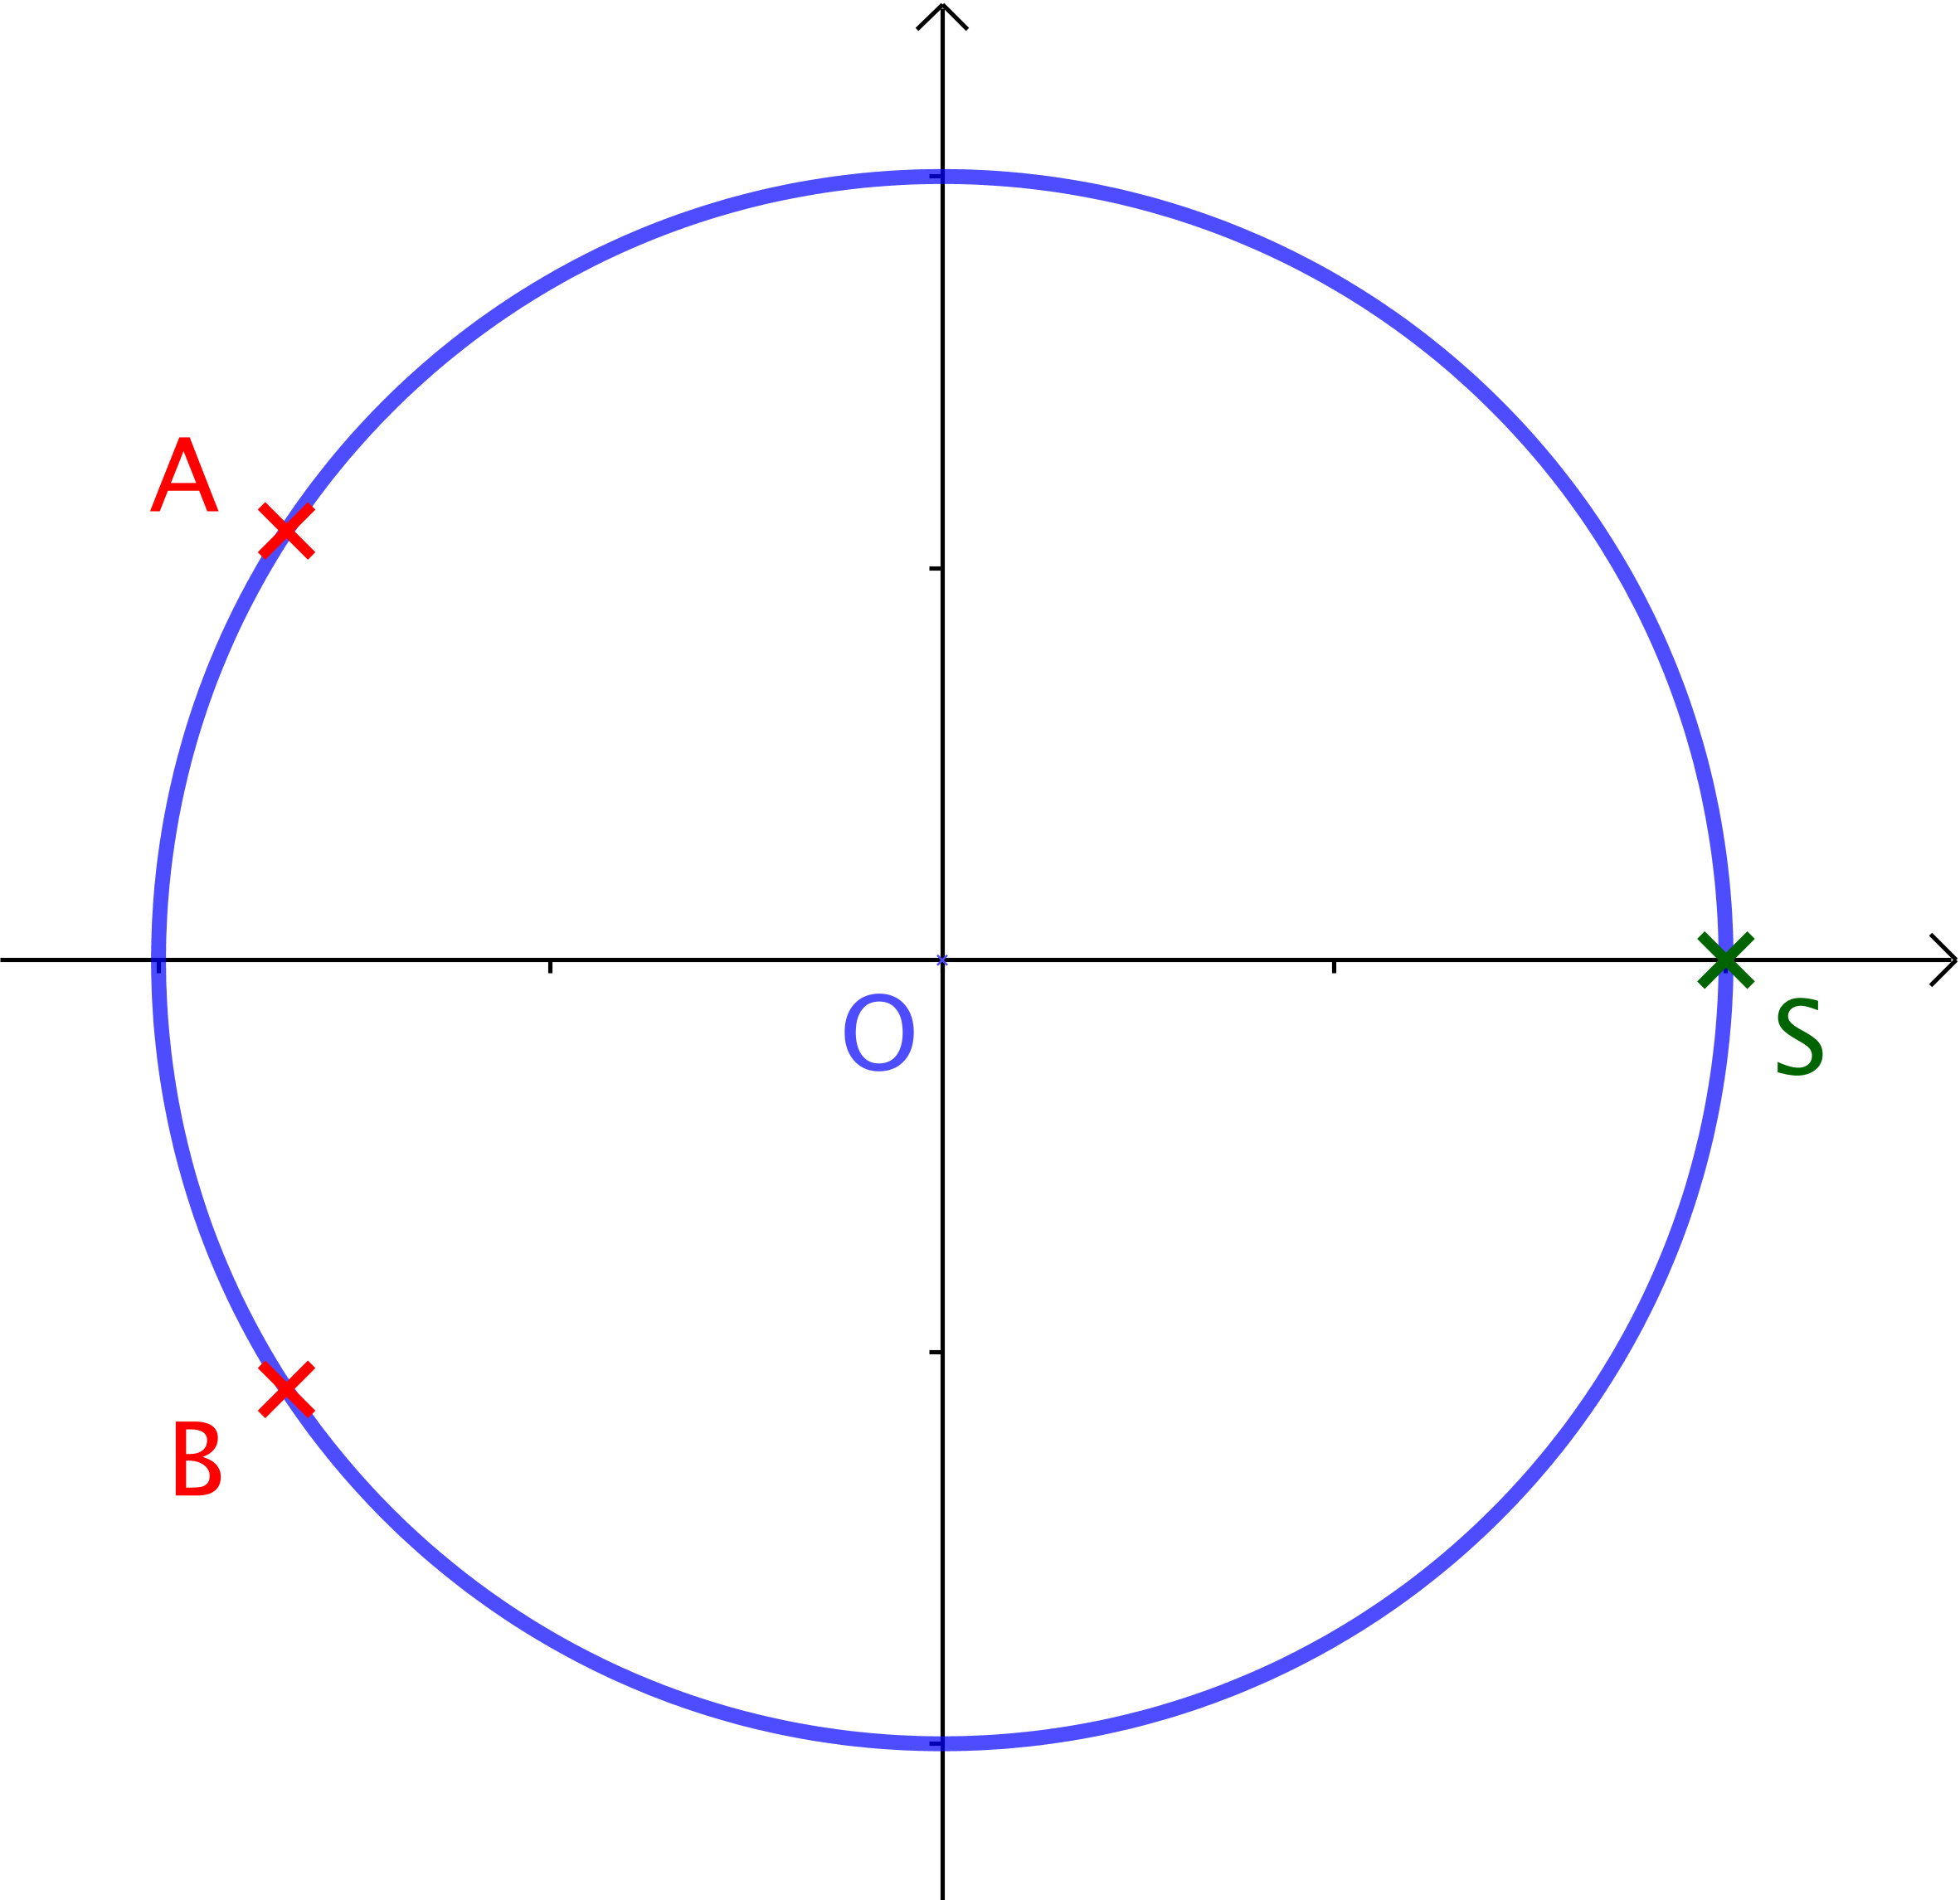
\includegraphics[scale = .75]{addition-on-ellipsis/conjecture/h-sym.png}}

	\columnbreak

	\fbox{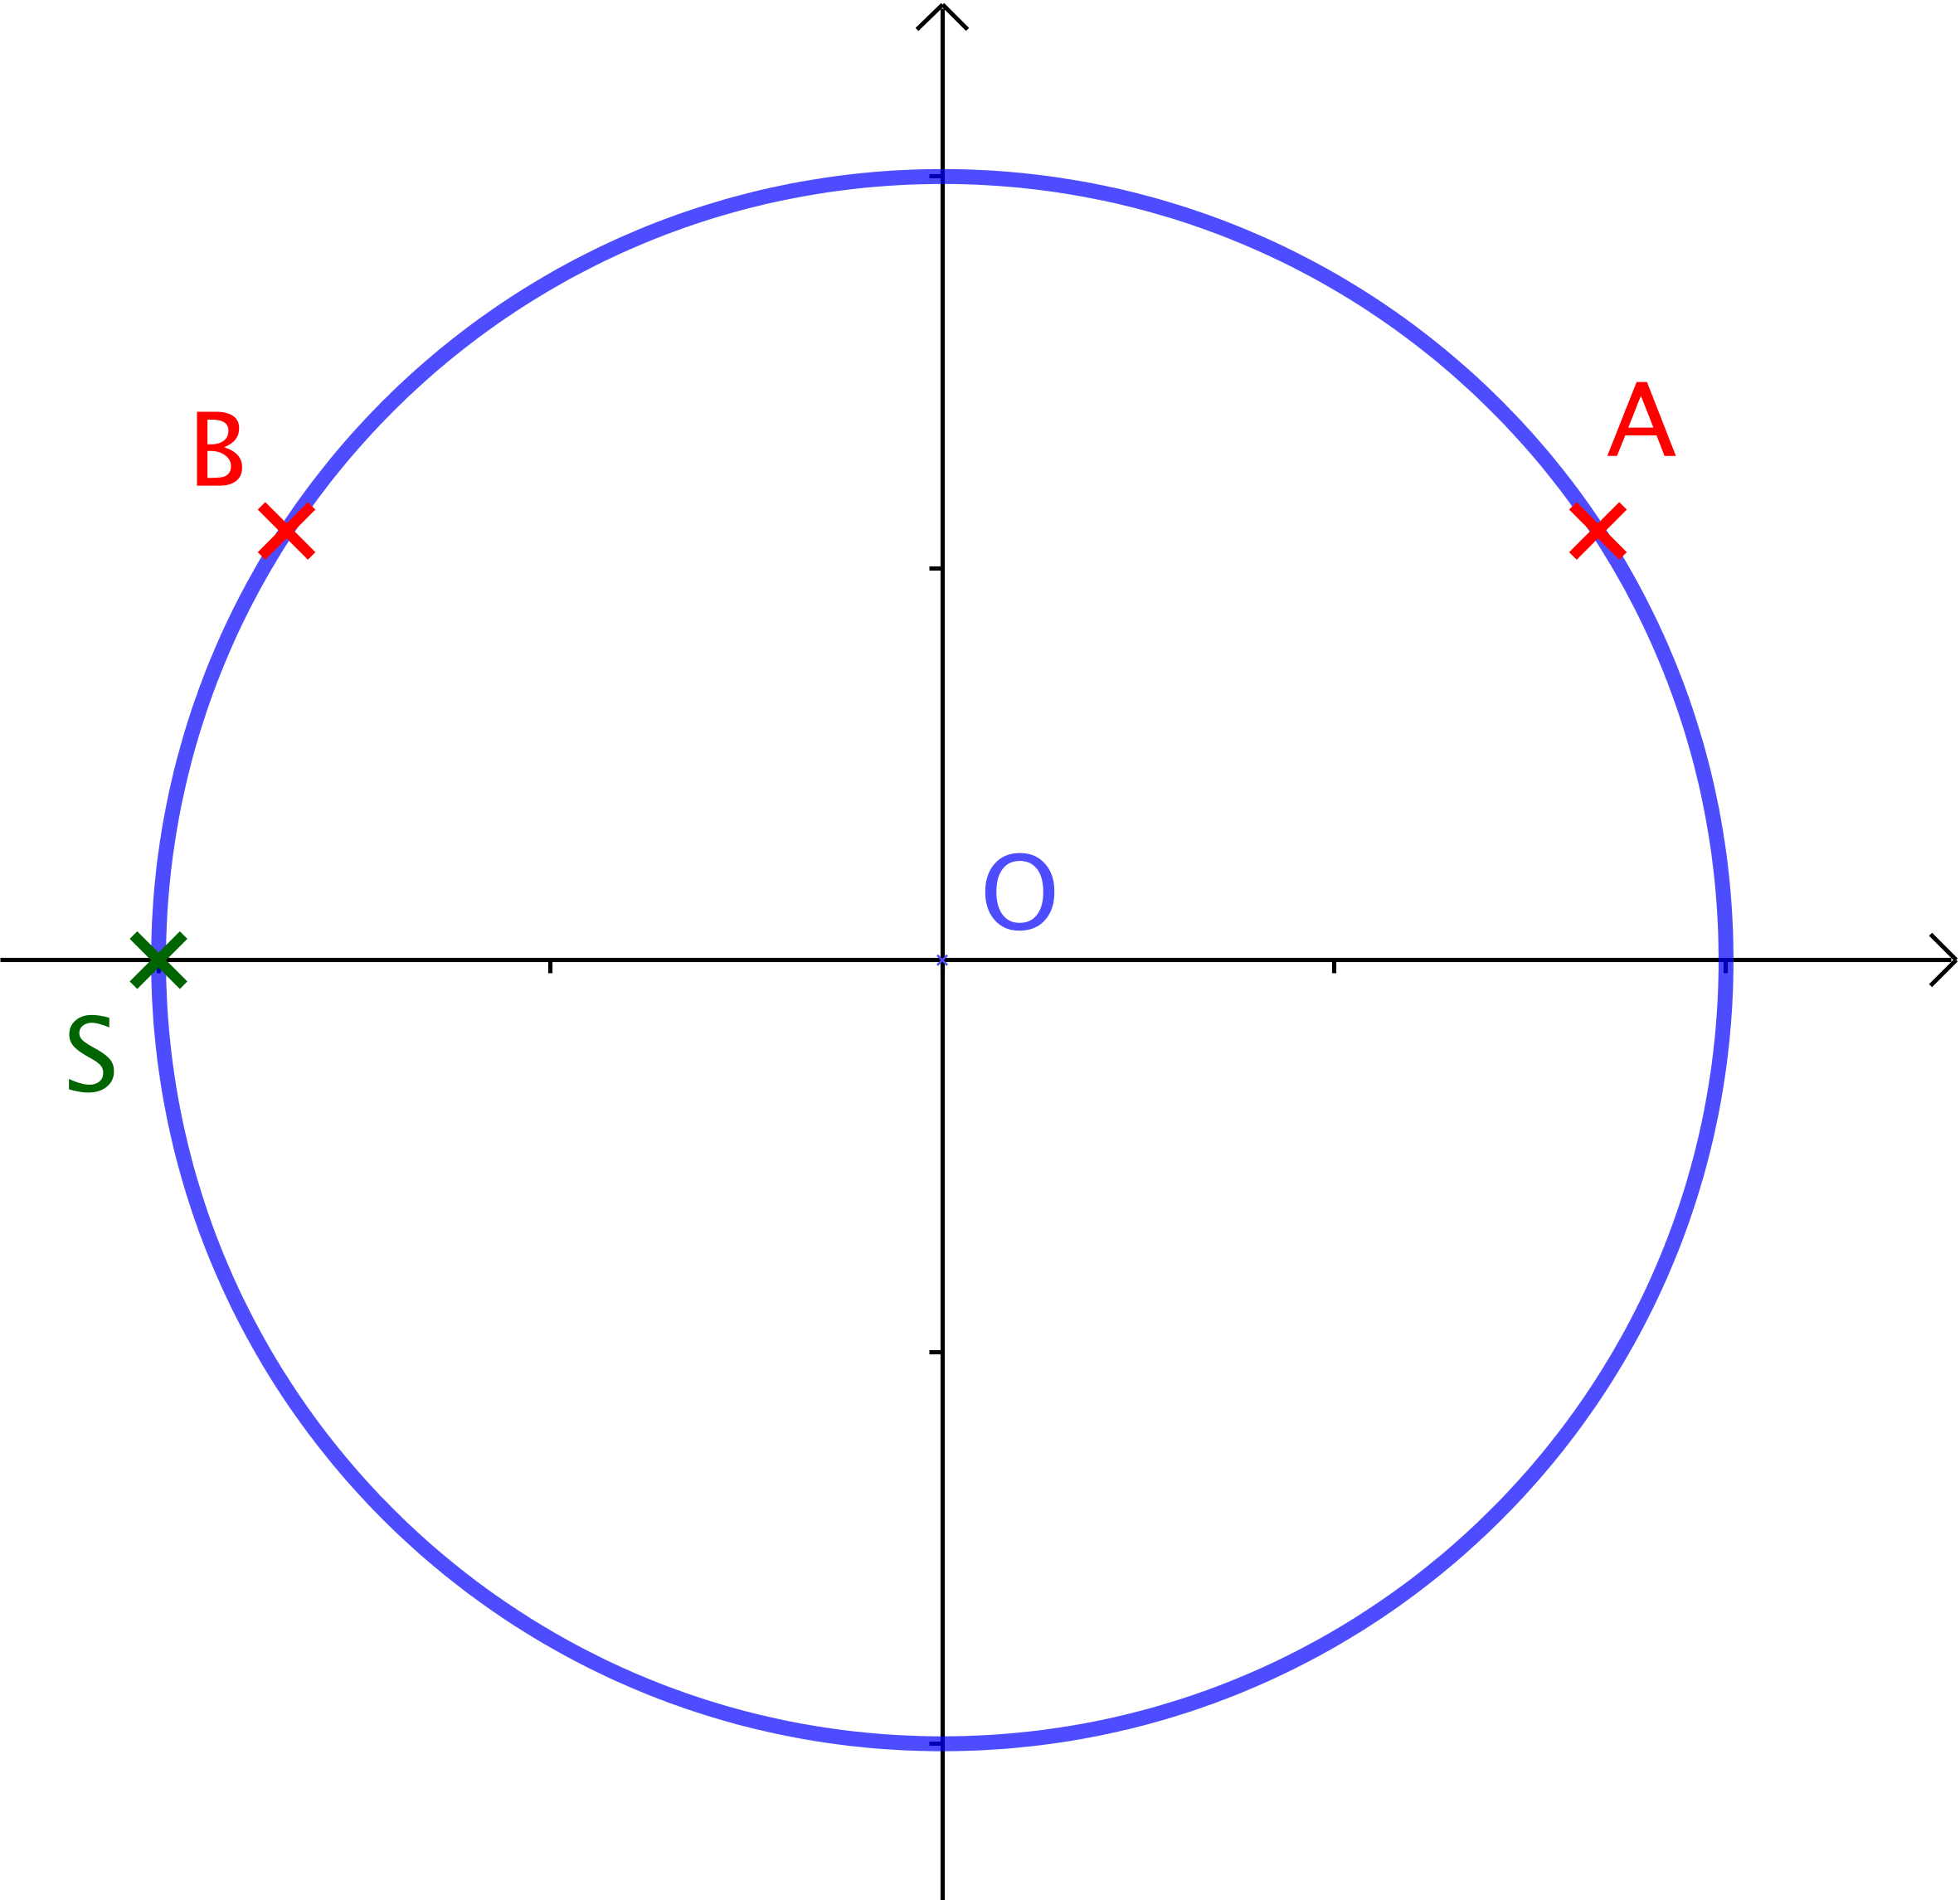
\includegraphics[scale = .75]{addition-on-ellipsis/conjecture/v-sym.png}}
\end{multicols}


\medskip

\begin{multicols}{2}
	\center

	\fbox{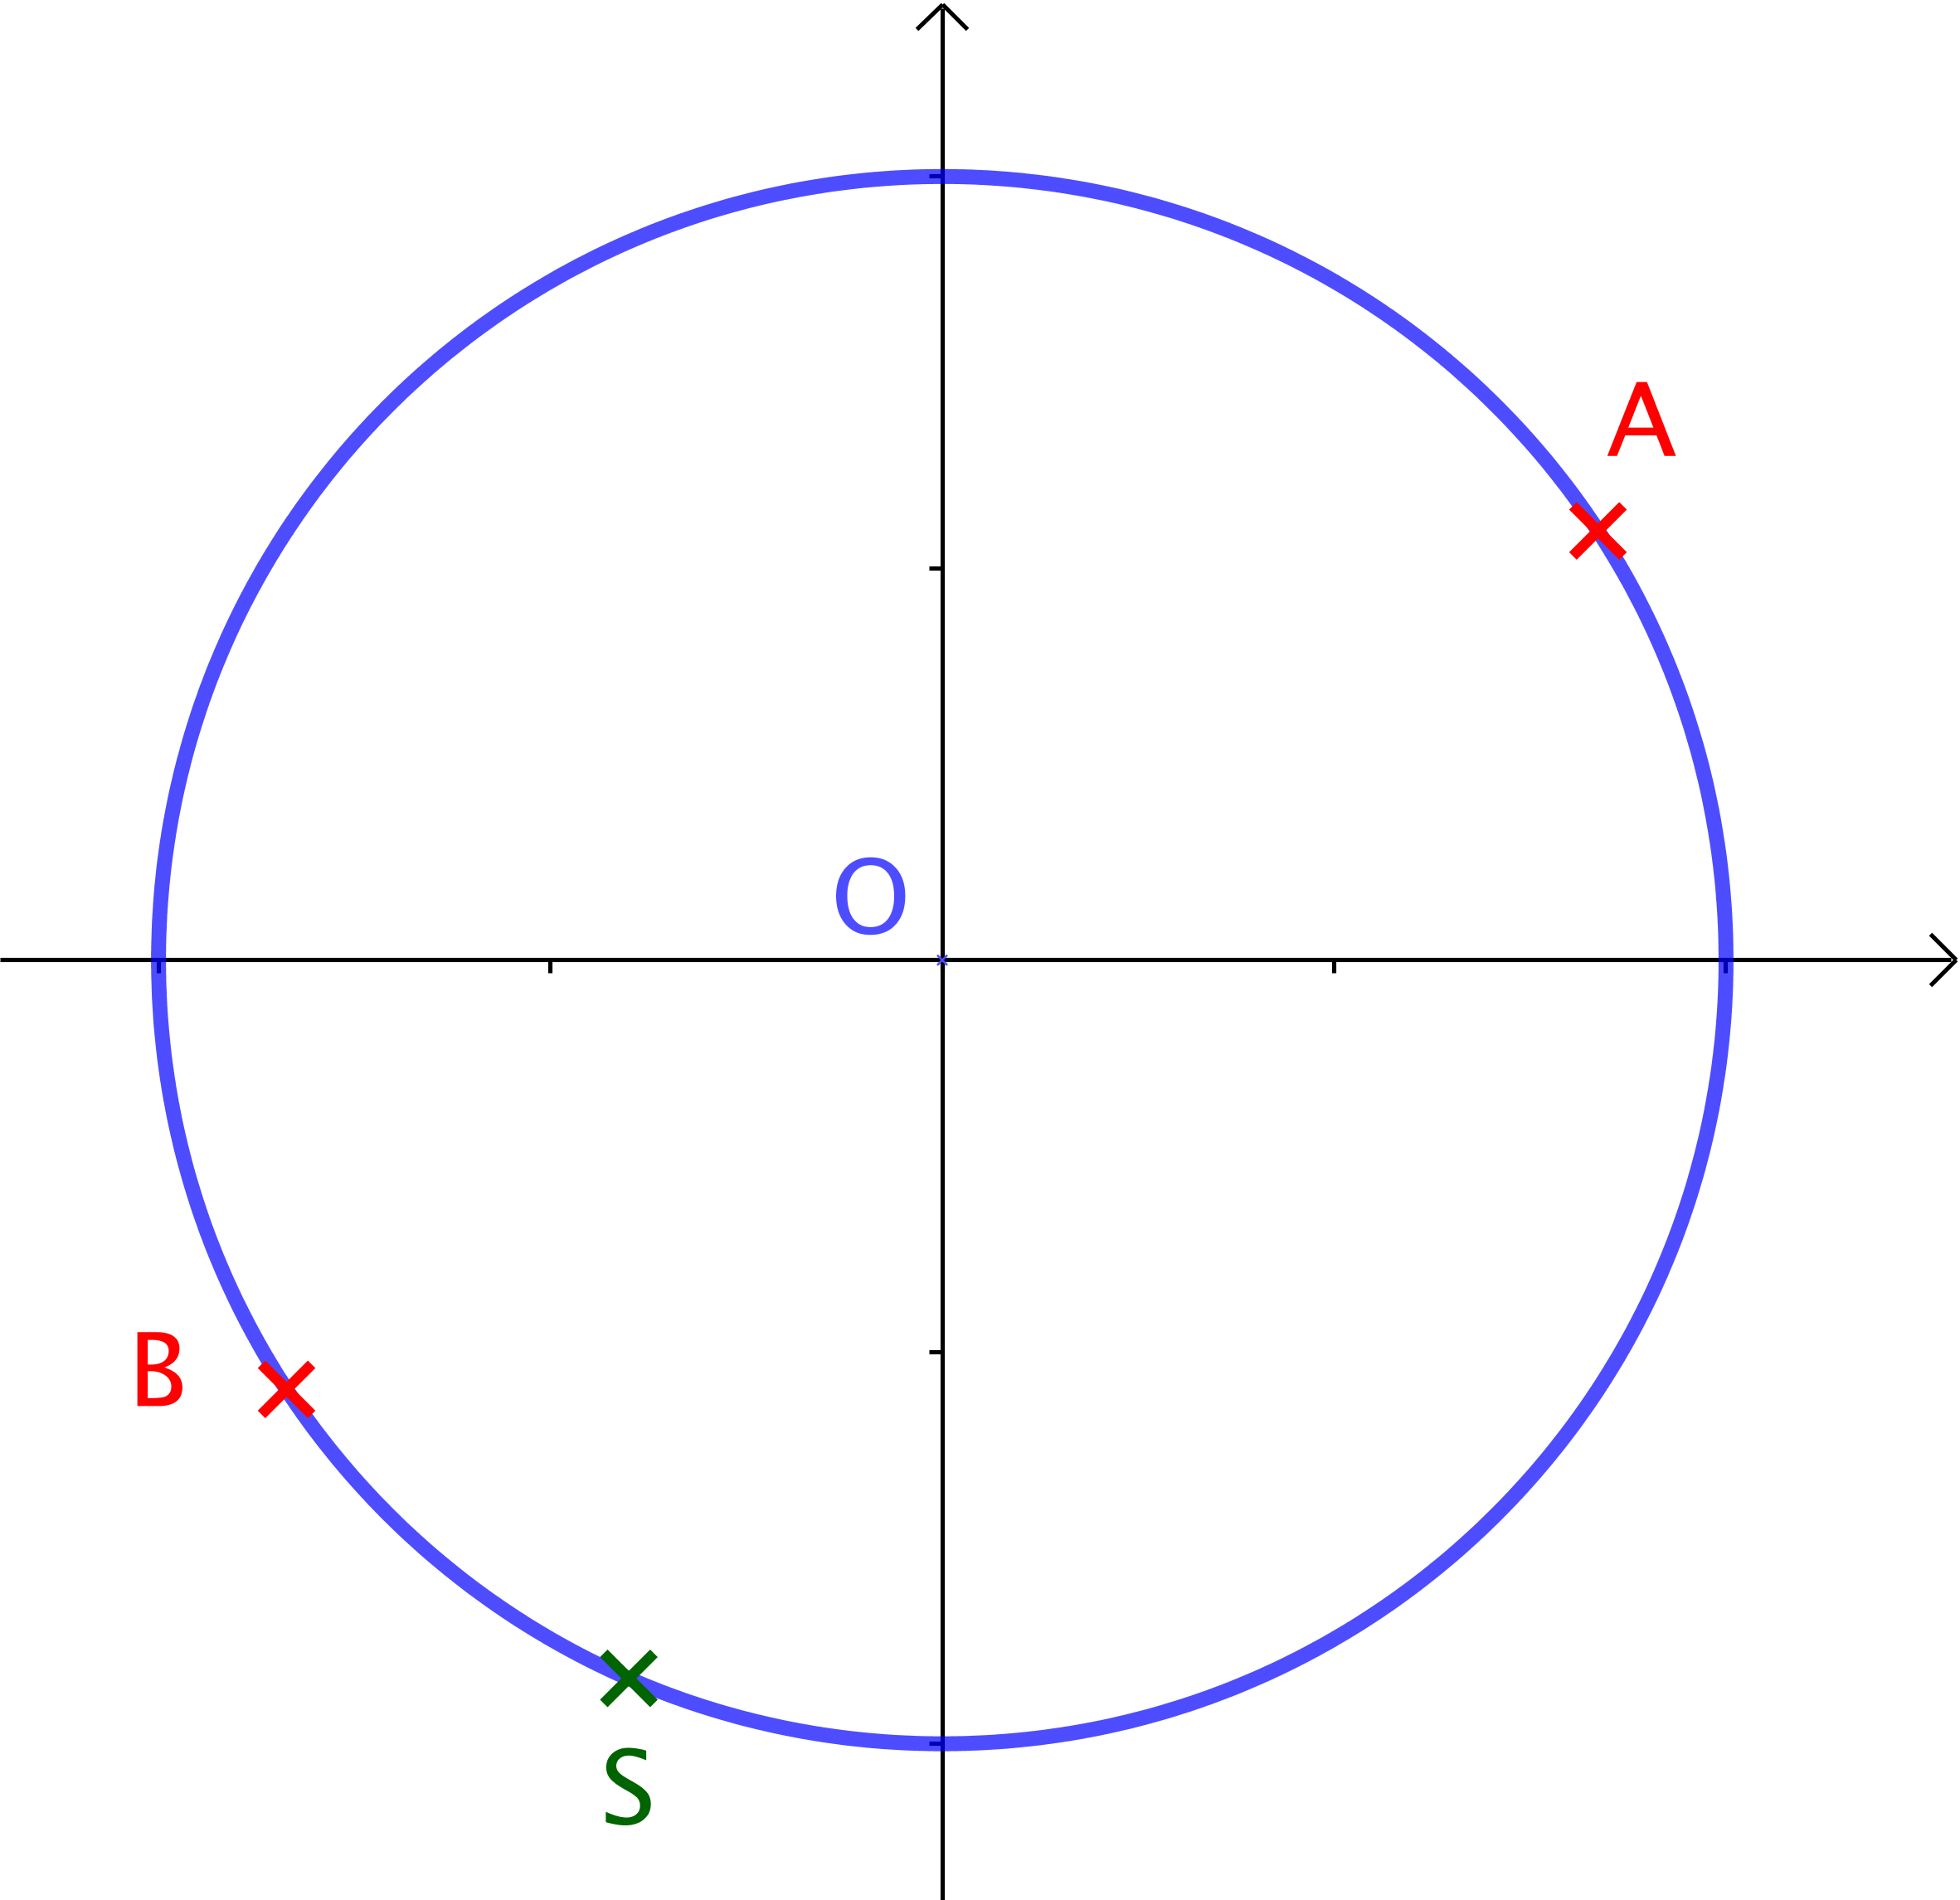
\includegraphics[scale = .75]{addition-on-ellipsis/conjecture/O-sym.png}}

	\columnbreak

	\fbox{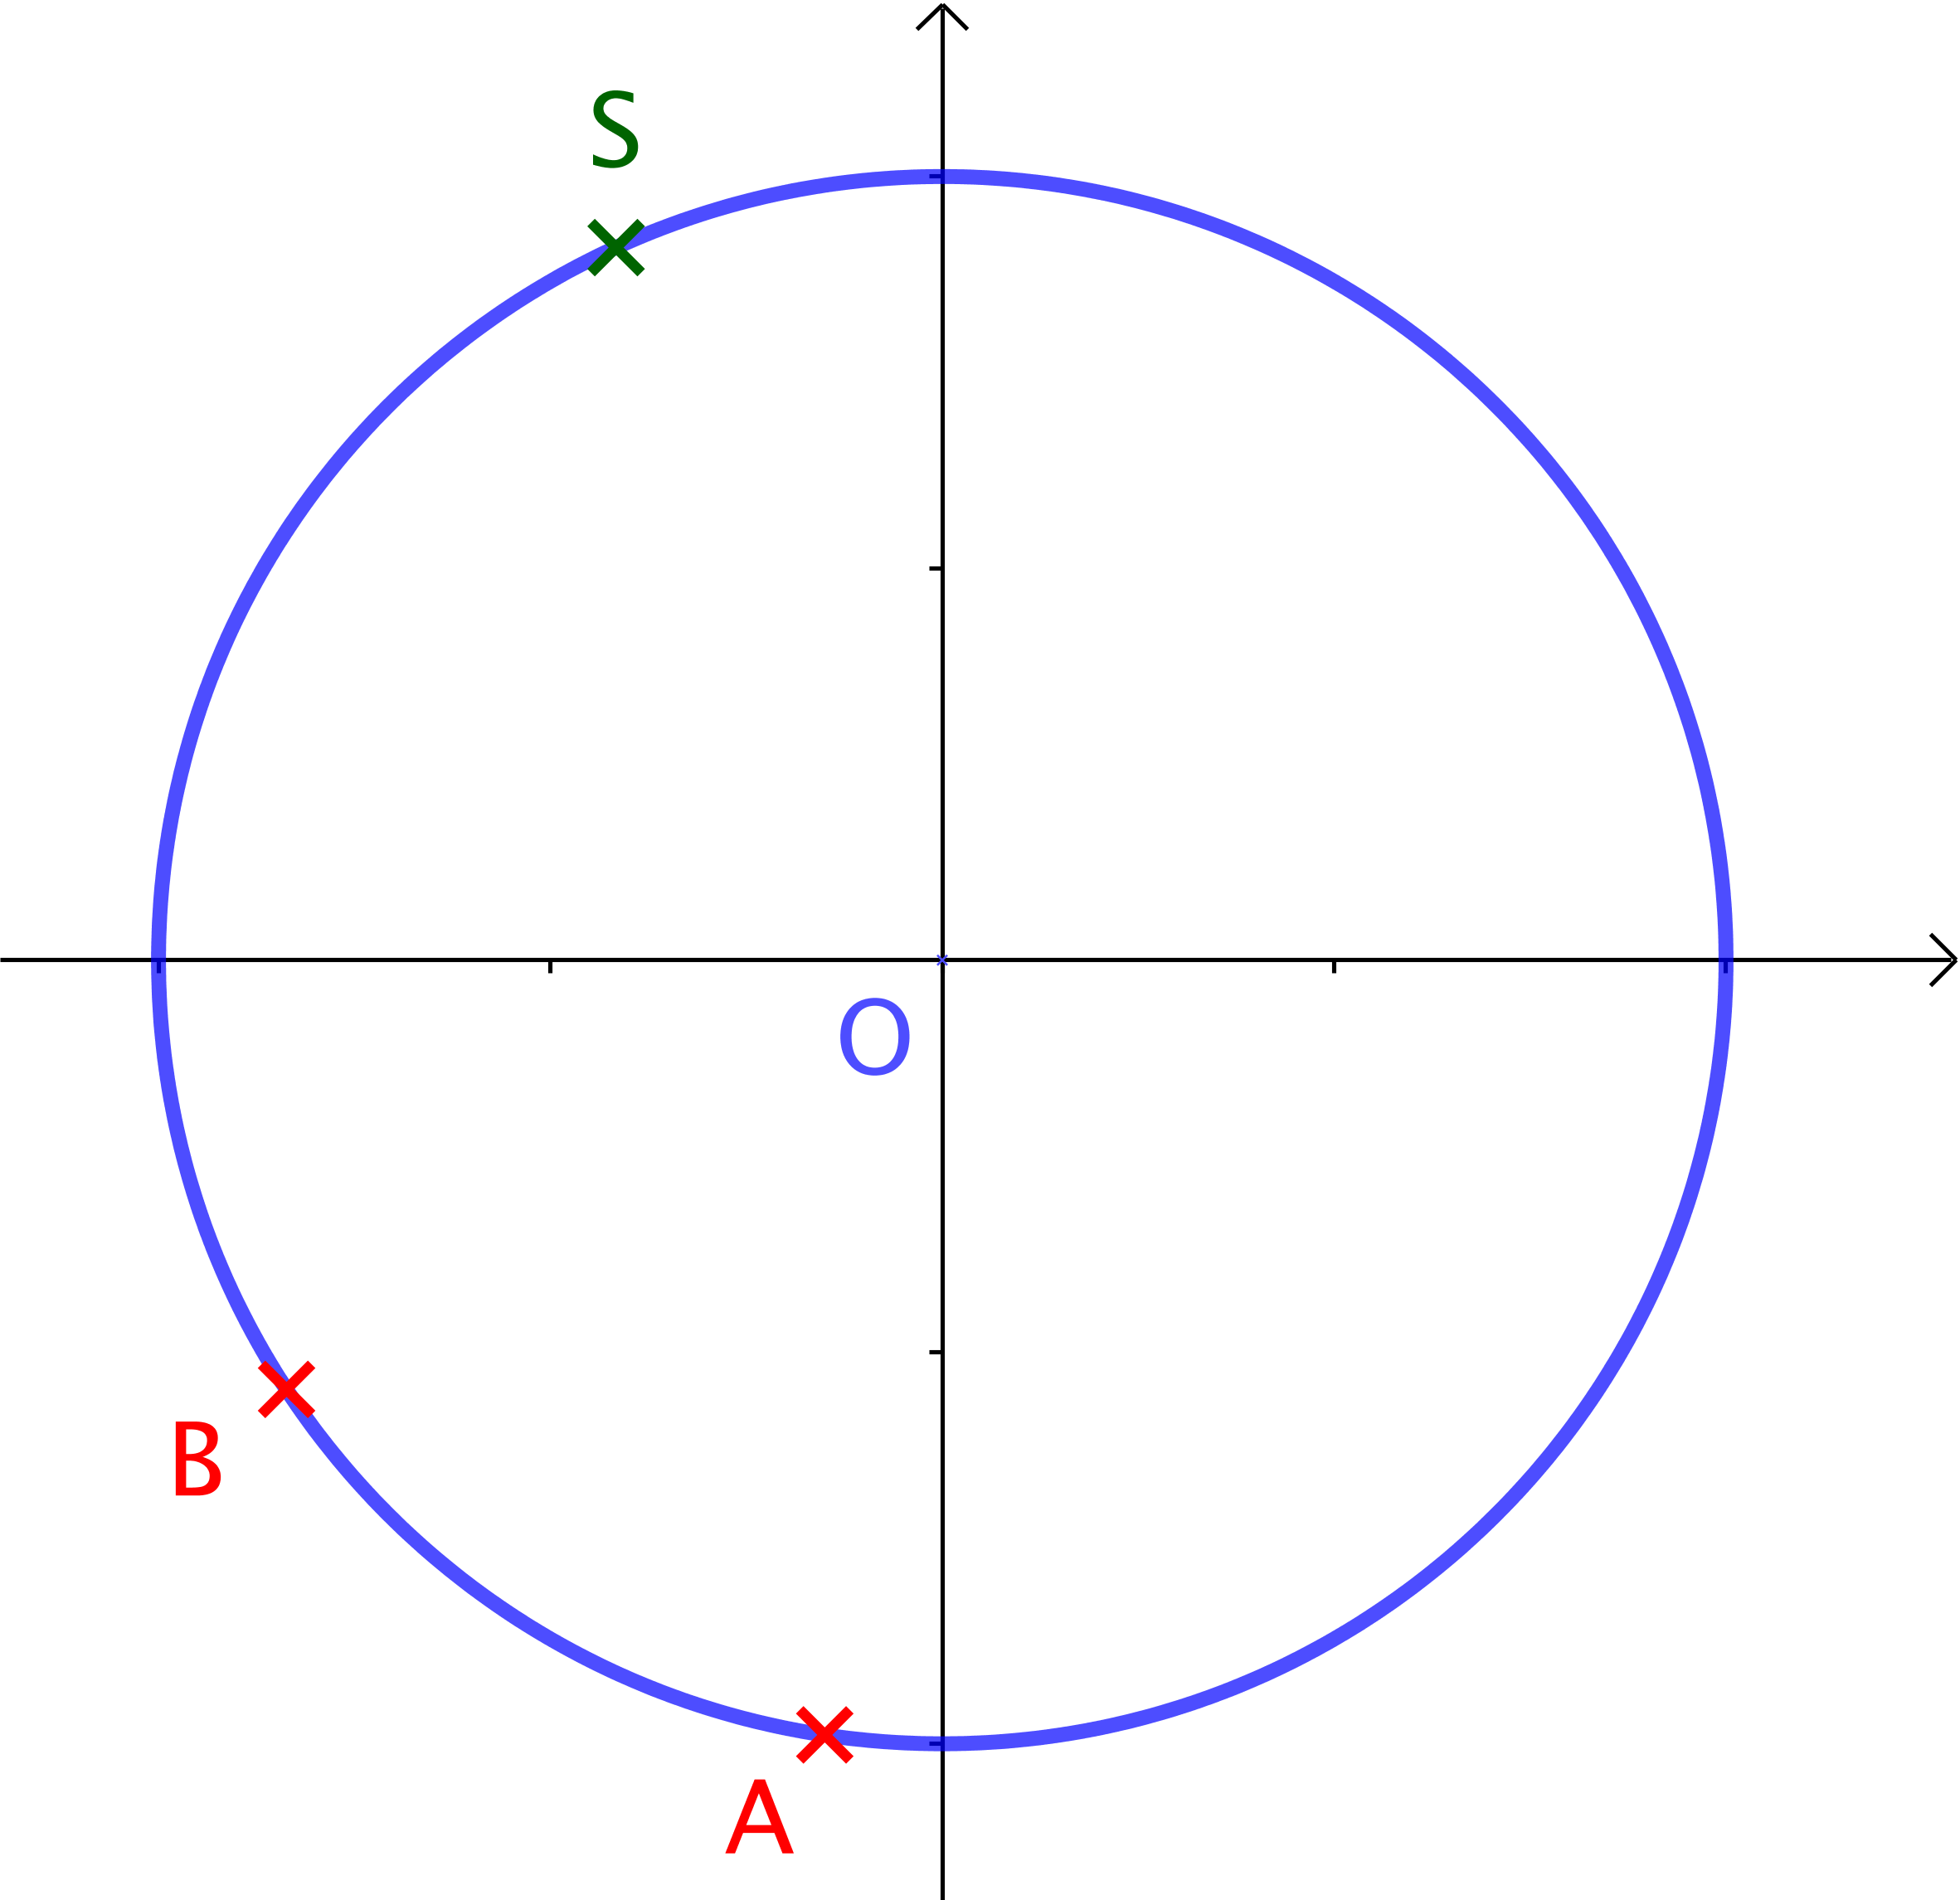
\includegraphics[scale = .75]{addition-on-ellipsis/conjecture/general.png}}
\end{multicols}


\newpage

Pour mieux voir ce qu'il se passe, il suffit de tracer quelques droites. Voici ce que cela donne.

\begin{multicols}{2}
	\center

	\fbox{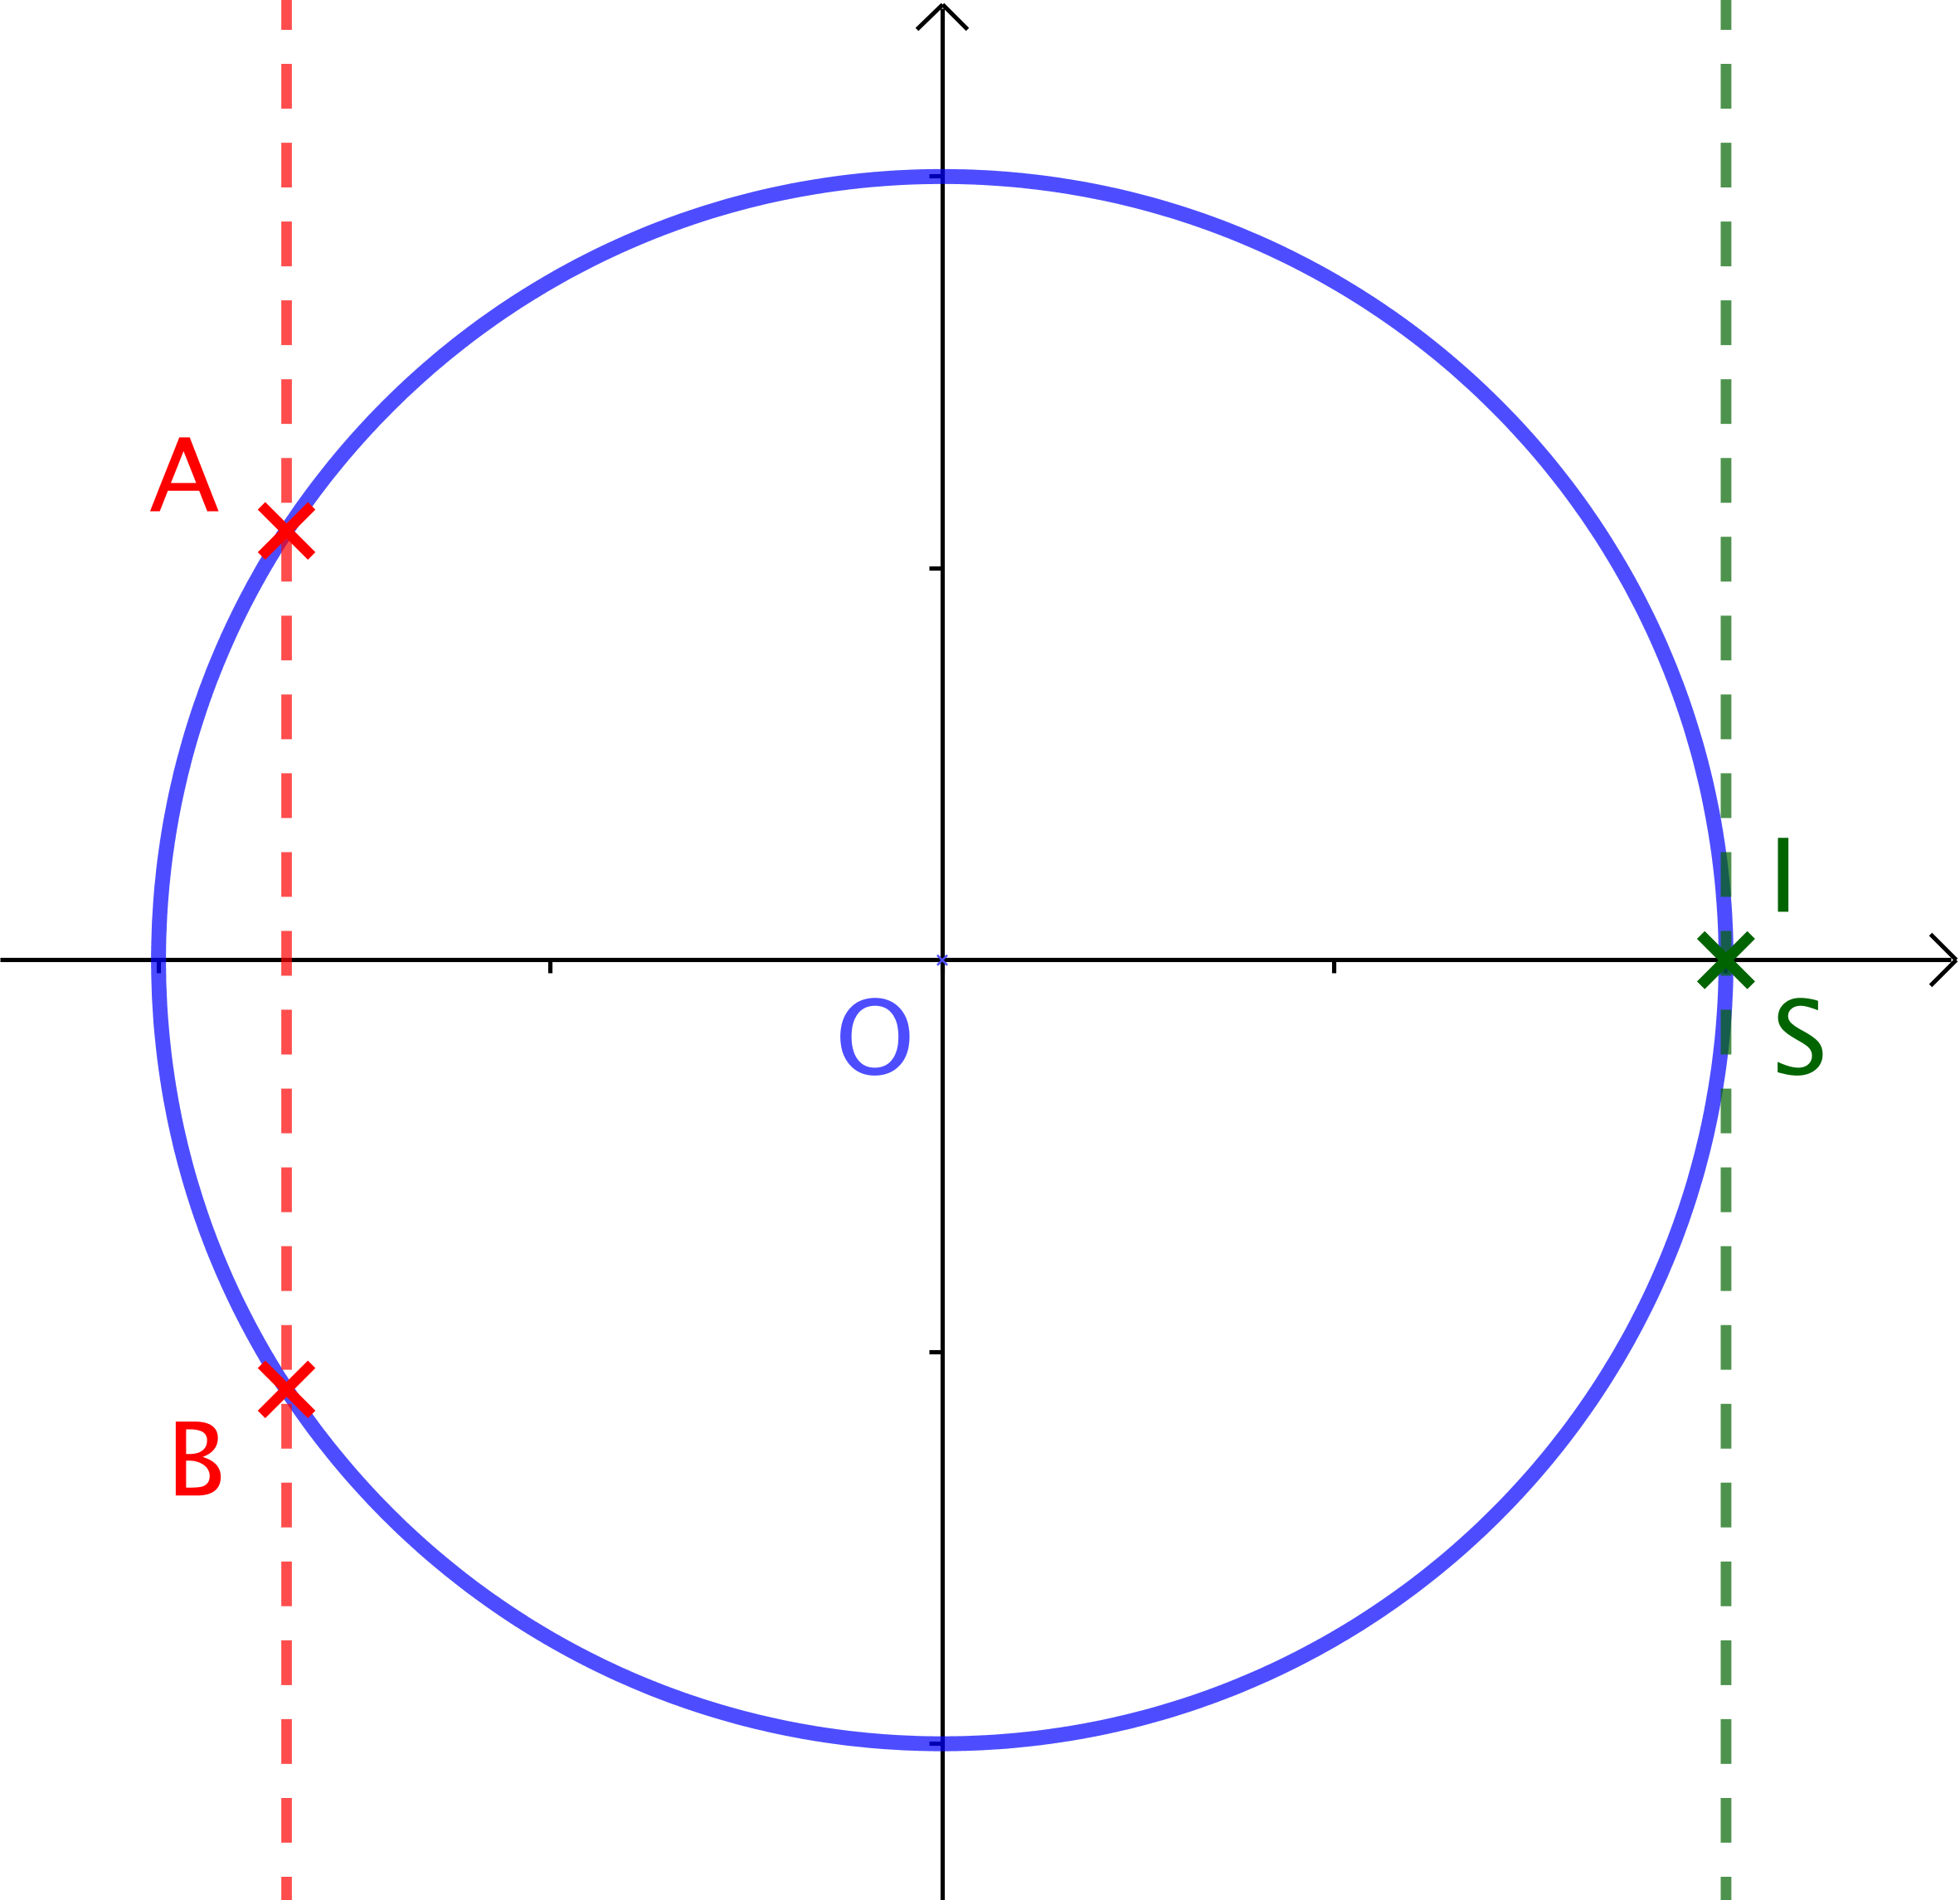
\includegraphics[scale = .75]{addition-on-ellipsis/conjecture/h-sym-with-lines.png}}

	\columnbreak

	\fbox{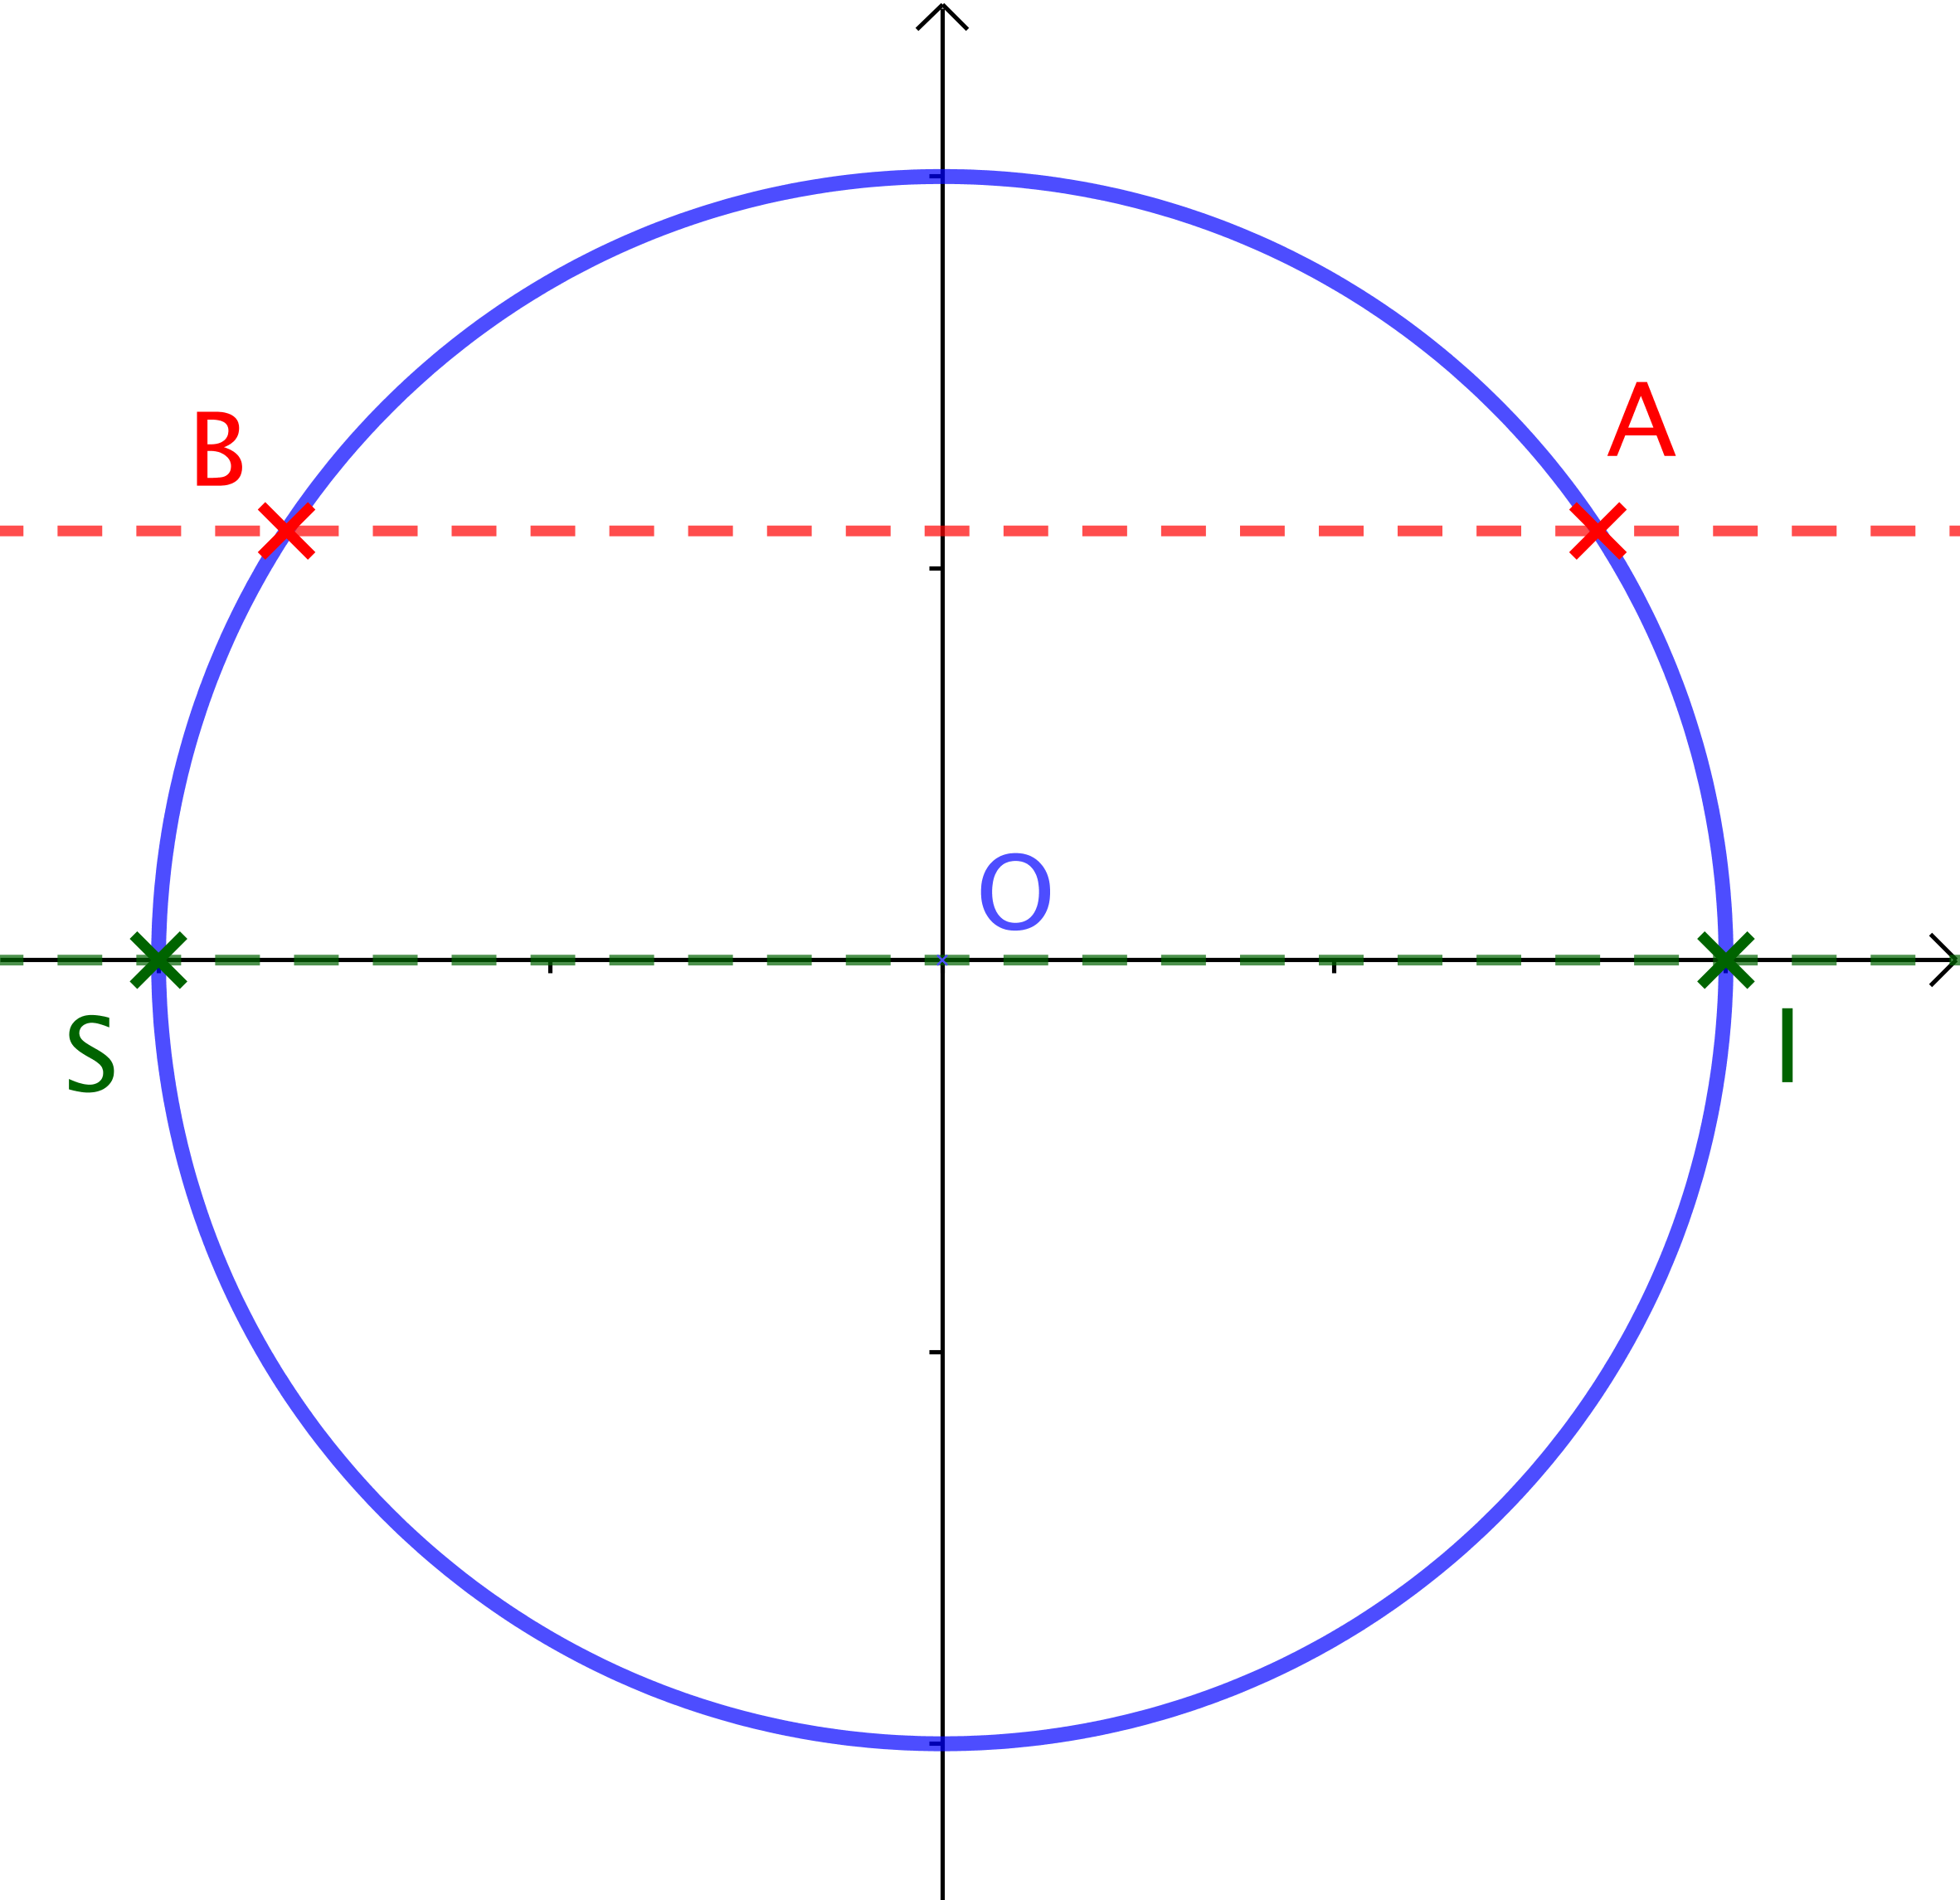
\includegraphics[scale = .75]{addition-on-ellipsis/conjecture/v-sym-with-lines.png}}
\end{multicols}


\medskip

\begin{multicols}{2}
	\center

	\fbox{\includegraphics[scale = .75]{addition-on-ellipsis/conjecture/o-sym-with-lines.png}}

	\columnbreak

	\fbox{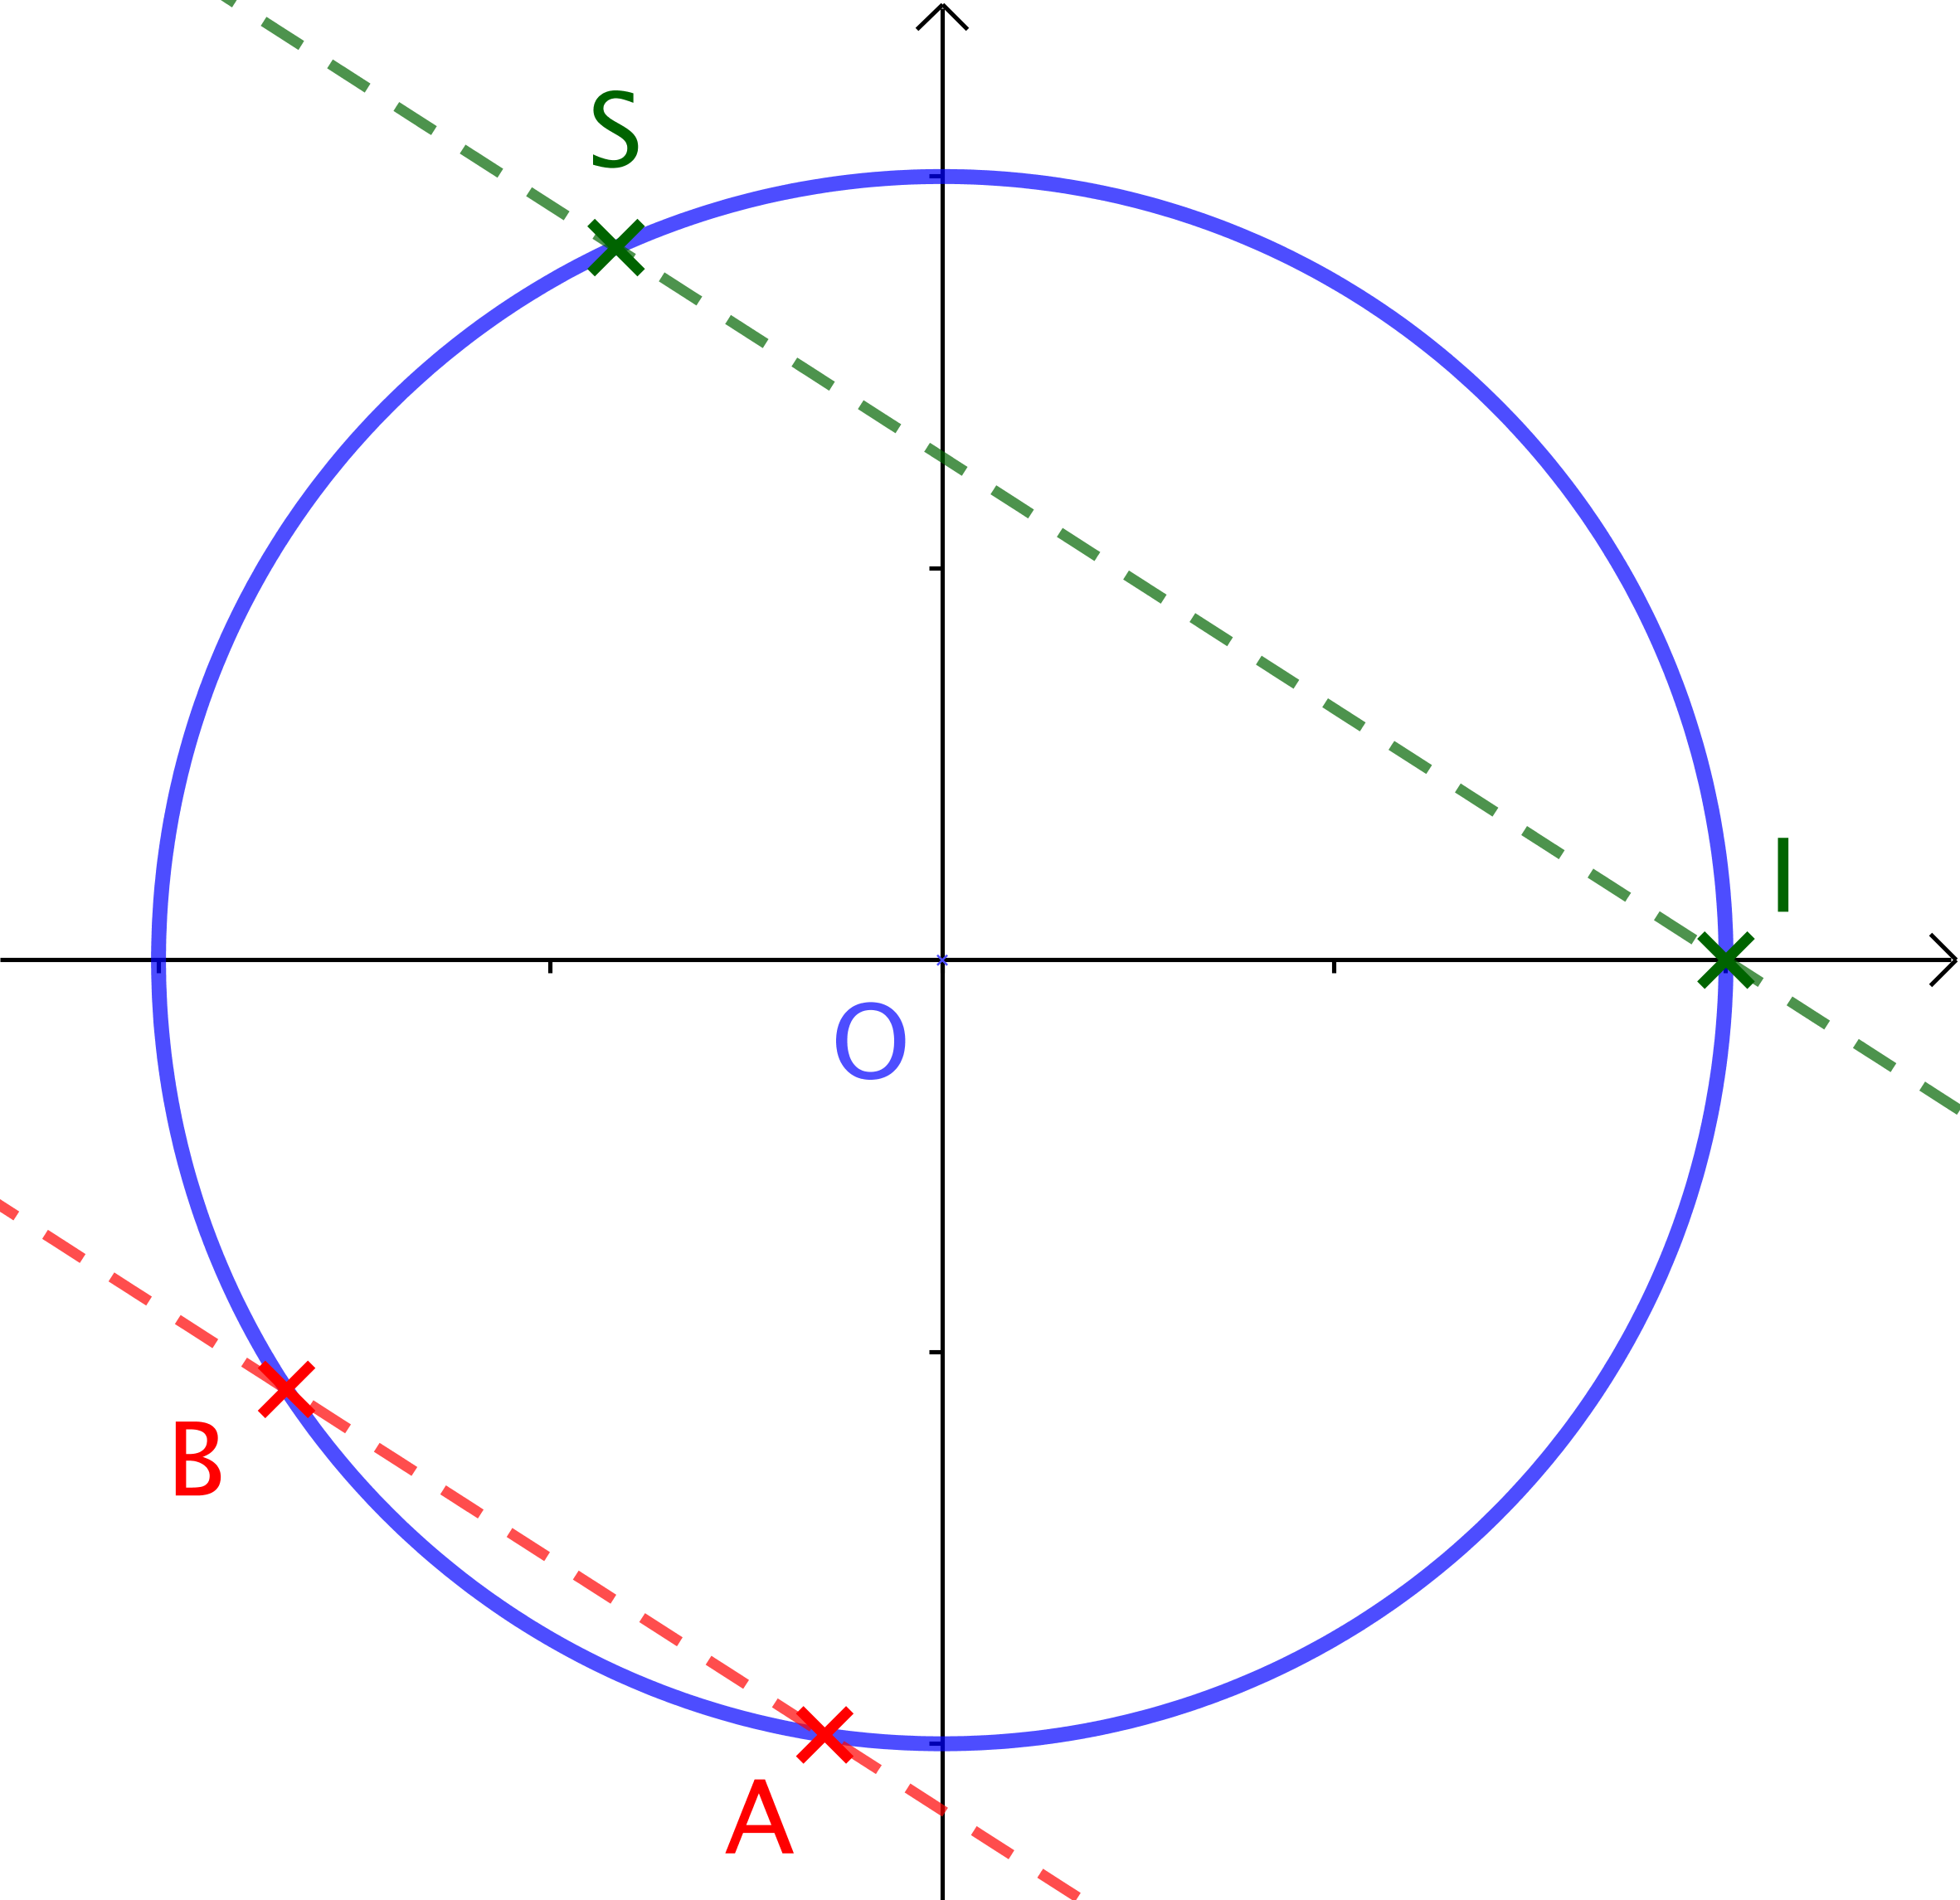
\includegraphics[scale = .75]{addition-on-ellipsis/conjecture/general-with-lines.png}}
\end{multicols}


Il devient évident de conjecturer que le point $S$ se construit géométriquement comme suit.

\begin{enumerate}
	\item \label{point-1} Si $A \neq B$ alors on construit la parallèle à $(AB)$ passant par $I$ . 
	Si cette parallèle n'est pas tangente au cercle alors le point $S$ est le second point d'intersection de cette parallèle avec le cercle, sinon $S = I$ .
	Notons que dans le second cas, c'est à dire si $x_A = x_B$ et $y_A = -y_B$ , alors $S = I$ peut être vu comme un point d'intersection \squote{double}.

	\item Si $A = B$ , on procède comme au point (\ref{point-1}) mais avec la parallèle à la tangente en $A$ au cercle. Intuitivement, cette situation consiste à faire \emph{\og tendre \fg} $A$ vers $B$ 
	\footnote{
		Nous évitons les arguments faisant appel à l'analyse afin de rester dans un cadre géométrique le plus général possible.
	}.
\end{enumerate}


\medskip

Dans ce qui suit nous allons valider cette conjecture de trois façons en allant du plus brutal au plus élégant.

\begin{enumerate}
	\item La 1\iere{} méthode passe assez brutalement via les critères de colinéarité et d'orthogonalité dans un plan.
	
	\item La 2\ieme{} méthode utilise les nombres complexes avec des calculs faciles à mener.
	
	\item La 3\ieme{} méthode, sûrement la plus élégante, est purement géométrique.
\end{enumerate}
